\documentclass[a4paper,10pt]{article}
\usepackage[utf8]{inputenc}
\usepackage{amsmath}
\usepackage{amsfonts}
\usepackage{hyperref}
\usepackage{tikz}
\usepackage{pgfplots}
\pgfplotsset{compat=1.17}
\usepackage{microtype}

\title{Arbitrage Pricing Theory (APT) Models \& Multifactor Models}
\author{Nathan NDJOLI - \href{mailto:nathan.ndjoli1@gmail.com}{nathan.ndjoli1@gmail.com}}
\date{July 2024}

\begin{document}

\maketitle

\section*{The Capital Asset Pricing Model (CAPM)}

\noindent The Security Market Line (SML) is a graphical representation that illustrates the relationship between the expected return of assets and their systematic, non-diversifiable risk, which is measured by beta (\(\beta\)). This line is a key concept in the Capital Asset Pricing Model (CAPM) and serves to show how the risk of an asset is compensated by its expected return. Below is a diagram illustrating the SML and its components, with the expected return on the y-axis and the beta on the x-axis. \\

\begin{figure}[ht]
\centering
\begin{tikzpicture}[scale=1]
    \begin{axis}[
        width=\textwidth,
        height=0.5\textwidth,
        axis lines=middle,
        xlabel={$\beta_i$},
        ylabel={$E(R_i)$},
        xmin=0, xmax=7.75, ymin=0, ymax=9.75,
        xtick={0},
        ytick={0},
        clip=false,
        domain=0:7.75,
        samples=100,
        every axis x label/.style={at={(ticklabel* cs:1)}, anchor=west},
        every axis y label/.style={at={(ticklabel* cs:1)}, anchor=south},
    ]
    \addplot[black, thick] {x+2} node[pos=1, anchor=west] {SML};
    \draw[dashed] (axis cs:3.875,0) -- (axis cs:3.875,5.875);
    \draw[dashed] (axis cs:0,5.875) -- (axis cs:3.875,5.875);
    \node[anchor=east] at (axis cs:-0.1,2) {$R_f$};
    \end{axis}
\end{tikzpicture}
\caption{Security Market Line }
\end{figure}

\noindent The diagram uses the following notations: \( R_i \) represents the return of asset \( i \), \( E(R_i) \) is the expected return of asset \( i \), \( R_f \) denotes the risk-free rate, \( E(R_M) \) is the expected market return, and \( \beta_i \) indicates the non-diversifiable risk of asset \( i \). \\

\noindent The return of asset \( i \) can be expressed as: \\
\[ R_i = \alpha_i + \beta_i R_M + \epsilon_i \] \\
\noindent Where \( \beta_i \) is calculated using: \\
\[ \beta_i = \frac{Cov(R_i, R_M)}{Var(R_M)} = \frac{\sigma_{i,M}}{\sigma_M^2} \] \\
\noindent Beta quantifies the asset's sensitivity to market movements. \\

\noindent The analytical expression of the SML is: \\
\[ E(R_i) = R_f + \beta_i (E(R_M) - R_f) \] \\
\noindent Which can be rearranged to show the excess return: \\
\[ E(R_i) - R_f = \beta_i (E(R_M) - R_f) \] \\

\noindent In the context of an efficient portfolio, the beta of the portfolio (\( \beta_P \)) can be derived as follows: \\
\[ \beta_P = w \beta_M + (1 - w) \beta_f = w \] \\
\noindent Where \( w \) represents the weight of the market portfolio in the overall portfolio. Additionally, the variance of the portfolio (\( \sigma_P^2 \)) is given by: \\
\[ \sigma_P^2 = w^2 \sigma_M^2 = \beta_P^2 \sigma_M^2 \] \\
\noindent Thus, beta can also be expressed in terms of standard deviations: \\
\[ \beta_P = \frac{\sigma_P}{\sigma_M} \] \\

\noindent From this, we derive the Capital Market Line (CML), which relates the expected return of the portfolio (\( E(R_P) \)) to its total risk (\( \sigma_P \)): \\
\[ E(R_P) = R_f + \frac{\sigma_P}{\sigma_M} (E(R_M) - R_f) \] \\
\noindent This equation highlights that the risk of an efficient portfolio is entirely non-diversifiable risk: \\
\[ \sigma_P = \beta_P \sigma_M \] \\
\

\section{Criticisms of the CAPM}

\noindent The Capital Asset Pricing Model (CAPM) has faced numerous criticisms, particularly concerning the assumptions it makes about market conditions and investor behavior. One major criticism of the CAPM pertains to its assumption that returns are normally distributed. In real-world markets, asset returns often deviate from normality, exhibiting skewness and kurtosis. This leads to return distributions that can have fat tails or other anomalies, which the CAPM does not account for. This discrepancy between the assumed and actual distribution of returns can lead to inaccuracies in the model's predictions and its practical applications. \\

\noindent Another significant criticism is the assumption of homogeneous investor expectations. The CAPM posits that all investors share the same expectations regarding future returns and risks, an assumption that is far from realistic. In reality, investors have diverse risk preferences, investment horizons, and expectations based on their unique information sets and personal circumstances. This heterogeneity among investors means that their actions and reactions to market events can be vastly different, thereby challenging the uniformity assumed by the CAPM. \\

\noindent The CAPM also assumes that investors can borrow and lend unlimited amounts at the risk-free rate. This assumption is problematic because, in the real world, the conditions for borrowing and lending are not symmetric. Borrowing rates are typically higher than lending rates, reflecting the risk premium demanded by lenders. Moreover, access to borrowing is often constrained by factors such as creditworthiness and market conditions, which the CAPM does not consider. These limitations on borrowing can significantly impact an investor's ability to leverage their portfolio as the model assumes. \\

\noindent Roll's critique presents another profound challenge to the CAPM. According to this critique, the CAPM is inherently untestable because it requires the true market portfolio, encompassing all investable assets, to be observed. In practice, such a comprehensive market portfolio is impossible to construct or observe. Empirical tests of the CAPM often use stock market indices as proxies for the market portfolio, but these indices represent only a subset of all possible investments. Consequently, the validity of empirical tests of the CAPM is questionable, as they do not account for the full scope of the market portfolio. \\

\section*{Arbitrage Pricing Theory (APT) Models}

\noindent The Arbitrage Pricing Theory (APT) relies on the existence of common risk factors. The return on asset \(i\) can be expressed as: \\
\[R_i = \alpha_i + \beta_1 F_1 + \beta_2 F_2 + \ldots + \beta_k F_k + \epsilon_i\] \\
\noindent Where: \\
\[E(F_1) = E(F_2) = \ldots = E(F_k) = E(\epsilon_i) = 0\] \\
\noindent And: \\
\[Cov(\epsilon_i, \epsilon_j) = Cov(F_k, F_l) = Cov(F_k, \epsilon_i) = 0\] \\

\noindent The APT can be depicted through a factor model, which illustrates how different factors influence asset returns. Below is an example: \\

\begin{figure}[ht]
\centering
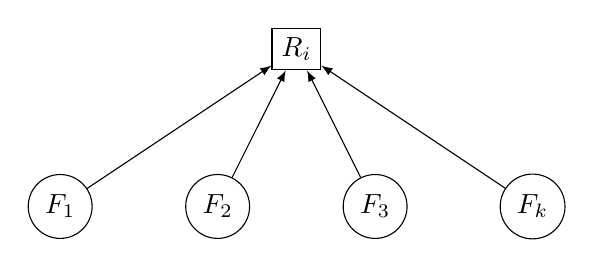
\begin{tikzpicture}
    \node at (0,0) [rectangle, draw] (Ri) {$R_i$};
    \node at (-3,-2) [circle, draw] (F1) {$F_1$};
    \node at (-1,-2) [circle, draw] (F2) {$F_2$};
    \node at (1,-2) [circle, draw] (F3) {$F_3$};
    \node at (3,-2) [circle, draw] (Fk) {$F_k$};

    \draw[-latex] (F1) -- (Ri);
    \draw[-latex] (F2) -- (Ri);
    \draw[-latex] (F3) -- (Ri);
    \draw[-latex] (Fk) -- (Ri);
\end{tikzpicture}
\caption{Multifactor Model illustrating influences on asset returns}
\end{figure}

\noindent Consider an example with a single risk factor. Suppose two risky assets with expected returns \(E(R_A) = 10\%\) and \(E(R_B) = 8\%\). The sensitivities of these assets to the risk factor are \(\beta_A = 0.8\) and \(\beta_B = 0.6\). We seek \(\alpha_0\) and \(\alpha_1\) such that \(E(R_i) = \alpha_0 + \alpha_1 \beta_i\). Given the expected returns and betas, we can set up the following system of equations to solve for \(\alpha_0\) and \(\alpha_1\): \\
\[0.10 = \alpha_0 + 0.8\alpha_1\] \\
\[0.08 = \alpha_0 + 0.6\alpha_1\] \\

\noindent Solving this system, we find: \\
\[\alpha_1 = \frac{0.10 - 0.08}{0.8 - 0.6} = \frac{0.02}{0.2} = 0.1\] \\
\noindent And: \\
\[\alpha_0 = 0.10 - 0.8 \times 0.1 = 0.10 - 0.08 = 0.02\] \\
\noindent Thus, the expected return equation becomes: \\
\[E(R_i) = 0.02 + 0.1 \beta_i\] \\

\noindent Arbitrage opportunities arise when there are mispricings in the market that allow for risk-free profits. In the context of APT, consider two portfolios. \\

\noindent First case: Consider a portfolio C with \(E(R_C) = 11\%\) and \(\beta_C = 0.7\). \\

\noindent Second case: Consider a portfolio C' with \(E(R_{C'}) = 9\%\) and \(\beta_{C'} = 0.7\). \\

\noindent Comparing these portfolios to the expected return equation \(E(R_i) = 0.02 + 0.1 \beta_i\), we find that for \(\beta_C = 0.7\): \\
\[E(R_C) = 0.02 + 0.1 \times 0.7 = 0.09\] \\
\noindent Since \(E(R_C) = 11\%\) is greater than 9\%, it suggests an arbitrage opportunity where portfolio C is overpriced. Conversely, if \(E(R_{C'}) = 9\%\), it is correctly priced according to the model. \\

\noindent The results of the APT show that, under the assumption of orthogonality: \[E(R_i) = \alpha_0 + \sum_{k=1}^K \alpha_k \beta_{i,k}\]\\ 
\noident In the presence of a risk-free asset with a return \(R_f\), we can write:\\ \[E(R_i) = R_f + \sum_{k=1}^K \alpha_k \beta_{i,k}\]\\

\noindent This generalization allows for multiple factors to explain asset returns, providing a more comprehensive model compared to CAPM, which only considers market risk. \\

\noindent The selection of factors in APT is crucial and can include macroeconomic variables, industry-specific factors, and other relevant variables. Each factor \(\alpha_k\) represents the risk premium associated with that factor. Investors are compensated for bearing systematic risk associated with each factor. Compared to the CAPM, which is a single-factor model focusing solely on market risk, the APT considers multiple factors. The CAPM is expressed as: \\
\[E(R_i) = R_f + \beta_i (E(R_M) - R_f)\] \\
\noindent with \(\alpha_M = E(R_M) - R_f\). This highlights that the CAPM is a single-factor model focusing solely on market risk, whereas APT considers multiple factors. 

\section*{Application of APT and Multifactor Models}

\noindent Arbitrage Pricing Theory (APT) and multifactor models play a crucial role in portfolio management by providing a comprehensive framework for assessing risk and return characteristics across various assets. These models incorporate both macroeconomic factors, such as GDP growth and inflation, and microeconomic factors, such as company earnings, to give a holistic view of asset returns. 

\noindent APT and multifactor models are used to capture the impact of these diverse factors on asset returns, enabling investors to make informed decisions based on a broader set of information. For instance, the return on an asset can be influenced by several macroeconomic factors, including economic growth rates, interest rates, and inflation, as well as microeconomic factors specific to the company, such as revenue growth, profit margins, and market share.\\

\begin{figure}[h]
\centering
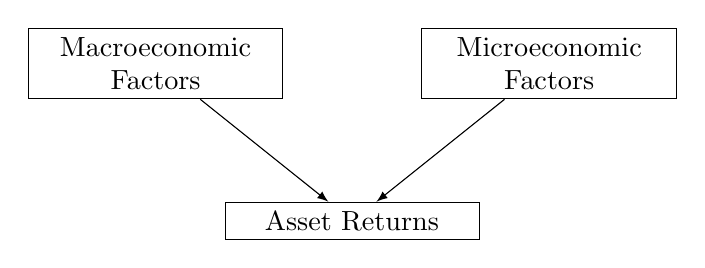
\begin{tikzpicture}
    \node at (0,0) [rectangle, draw, text width=3cm, align=center] (Macroeconomic) {Macroeconomic Factors};
    \node at (5,0) [rectangle, draw, text width=3cm, align=center] (Microeconomic) {Microeconomic Factors};
    \node at (2.5,-2) [rectangle, draw, text width=3cm, align=center] (AssetReturns) {Asset Returns};

    \draw[-latex] (Macroeconomic) -- (AssetReturns);
    \draw[-latex] (Microeconomic) -- (AssetReturns);
\end{tikzpicture}
\caption{Influence of macro and microeconomic factors on asset returns}
\end{figure}\\


\section*{The Fama \&\ French Model}
\noindent The Fama and French three-factor model is particularly influential in understanding risk and return in equity markets. This model extends the Capital Asset Pricing Model (CAPM) by adding two additional factors to the market risk factor: size and value. The Fama and French model, formulated in 1992 and 1996, can be expressed as: \\
\[E(R_i) - R_f = \beta_M (E(R_M) - R_f) + \beta_{SMB} (E(S) - E(B)) + \beta_{HML} (E(H) - E(L))\] \\
\noindent In this equation, \(SMB\) (Small Minus Big) captures the size premium, reflecting the tendency for smaller companies to outperform larger ones. \(HML\) (High Minus Low) captures the value premium, indicating that companies with high book-to-market ratios tend to outperform those with low book-to-market ratios. 

\begin{figure}[h!]
\centering
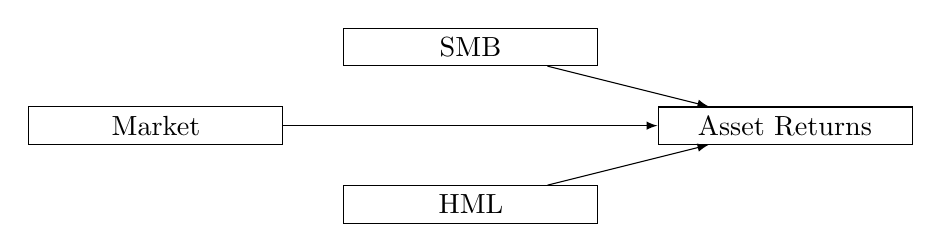
\begin{tikzpicture}
    \node at (0,0) [rectangle, draw, text width=3cm, align=center] (Market) {Market};
    \node at (4,1) [rectangle, draw, text width=3cm, align=center] (SMB) {SMB};
    \node at (4,-1) [rectangle, draw, text width=3cm, align=center] (HML) {HML};
    \node at (8,0) [rectangle, draw, text width=3cm, align=center] (Returns) {Asset Returns};

    \draw[-latex] (Market) -- (Returns);
    \draw[-latex] (SMB) -- (Returns);
    \draw[-latex] (HML) -- (Returns);
\end{tikzpicture}
\caption{Fama and French three-factor model}
\end{figure}

\section*{The Carhart Model}
\noindent The Carhart four-factor model, developed in 1997, builds on the Fama and French model by incorporating a momentum factor. This factor captures the tendency for stocks that have performed well in the past to continue performing well in the future, and for stocks that have performed poorly to continue underperforming. The Carhart model is expressed as: \\
\[E(R_i) - R_f = \beta_M (E(R_M) - R_f) + \beta_{SMB} (E(S) - E(B)) + \beta_{HML} (E(H) - E(L)) + \beta_{UMD} (E(U) - E(D))\] \\
\noindent Here, \(UMD\) (Up Minus Down) captures the momentum premium. This extension makes the model more robust by considering the performance trend of stocks over time.

\begin{figure}[ht]
\centering
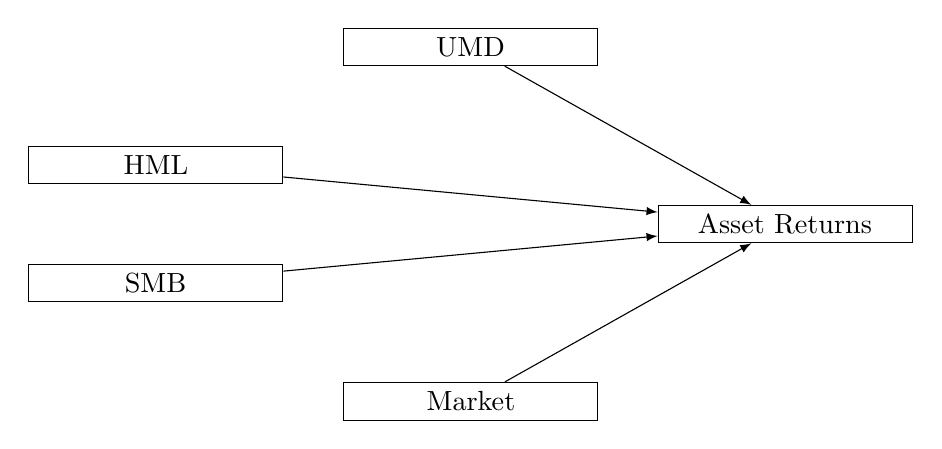
\begin{tikzpicture}
    \node at (4,0) [rectangle, draw, text width=3cm, align=center] (Market) {Market};
    \node at (0,1.5) [rectangle, draw, text width=3cm, align=center] (SMB) {SMB};
    \node at (0,3) [rectangle, draw, text width=3cm, align=center] (HML) {HML};
    \node at (4,4.5) [rectangle, draw, text width=3cm, align=center] (UMD) {UMD};
    \node at (8,2.25) [rectangle, draw, text width=3cm, align=center] (Returns) {Asset Returns};

    \draw[-latex] (Market) -- (Returns);
    \draw[-latex] (SMB) -- (Returns);
    \draw[-latex] (HML) -- (Returns);
    \draw[-latex] (UMD) -- (Returns);
\end{tikzpicture}
\caption{Carhart four-factor model}
\end{figure}

\noindent The application of these models in portfolio management enables investors to better understand the sources of risk and return in their portfolios. By incorporating multiple factors, these models provide a more nuanced view of asset performance, allowing for more effective risk management and investment strategies. They help investors to identify and capitalize on the various risk premiums present in the market, thereby enhancing their ability to achieve superior risk-adjusted returns. \\

\noindent Overall, APT and multifactor models offer a sophisticated approach to analyzing asset returns by considering a broad array of factors that influence market performance. They move beyond the single-factor approach of the CAPM, providing a richer framework for understanding and managing investment risks and opportunities. \\

\end{document}